\documentclass{article}

% Course adaptation of the instructor-supplied NeurIPS 2021 template (style file unchanged).
% Build from this directory:  latexmk -pdf -interaction=nonstopmode Credit_Default_Report.tex
% Figures are read from ../results/figures (PDF), produced by scripts/09_report_figures.py.
% Body + references must fit in 7 pages; appendices are not counted.
\PassOptionsToPackage{numbers,sort&compress}{natbib}
\usepackage[preprint]{neurips_2021}
\usepackage[utf8]{inputenc}
\usepackage[T1]{fontenc}
\usepackage{amsmath,amsfonts,amssymb}
\usepackage{booktabs,tabularx,array,multirow}
\usepackage{graphicx}
\usepackage{subcaption}
\usepackage{caption}
\usepackage{microtype}
\usepackage{xurl}
\usepackage[hidelinks]{hyperref}
\usepackage{xcolor}
\renewcommand{\bibfont}{\small}
\setlength{\bibsep}{0.5pt}
\graphicspath{{../results/figures/}}

% Editing marks: remove before submission. \todo{} prints in red; \draft{} prints in grey.
\newcommand{\todo}[1]{\textcolor{red}{[TODO: #1]}}
\newcommand{\draft}[1]{\textcolor{gray}{#1}}

\makeatletter
\renewcommand{\@noticestring}{MH6805 Machine Learning in Finance.\quad Group project final report.}
\makeatother
\hypersetup{
  pdftitle={Credit Card Default Prediction: Comparing Classification Models and Decision Thresholds},
  pdfauthor={Shi Xi, Li Erteng, Jiang Chengrui},
  pdfsubject={MH6805 group project final report}
}

\newcommand{\AP}{\mathrm{AP}}
\newcommand{\FN}{\mathrm{FN}}
\newcommand{\FP}{\mathrm{FP}}

\title{Credit Card Default Prediction:\\Comparing Classification Models\\and Decision Thresholds}
\author{%
  Shi Xi \qquad Li Erteng \qquad Jiang Chengrui\\
  Nanyang Technological University\\
  MH6805 Machine Learning in Finance\\
  \texttt{\href{https://github.com/ishixi233/Credit-MLoF}{github.com/ishixi233/Credit-MLoF}}
}
\date{}

\begin{document}
\maketitle
\thispagestyle{plain}

\begin{abstract}
A credit-risk classifier is operated through a threshold, so the model that ranks defaulters best need not minimise the cost of a given decision. We study this gap on the UCI Default of Credit Card Clients data (30{,}000 Taiwanese cardholders, 22.1\% default) by comparing six classifiers under one protocol: a stratified 70/30 split, five-fold cross-validation for configuration selection by average precision (AP), out-of-fold selection of the threshold that minimises a weighted error $r\cdot\FN+\FP$ for $r\in\{1,2,3,5,10\}$ with 5:1 as the pre-specified illustrative scenario, and a single evaluation of the frozen models on the test set, with calibration curves and Brier scores. Random Forest achieves the highest test AP (0.561; paired bootstrap intervals exclude every competitor) and the lowest cost for $r\ge3$, but for $r\le2$ it is statistically indistinguishable from Logistic Regression, AdaBoost and a depth-5 Decision Tree. Threshold choice matters more than model choice: at the default threshold of 0.5 every model is more expensive than flagging everyone when $r=5$, whereas cost-selected thresholds reduce cost by 23--29\%. Gaussian Naive Bayes ranks acceptably (ROC-AUC 0.73) but its probabilities are worse than the base rate (Brier skill $-0.67$), showing why calibration must be checked before thresholds are read as probabilities.
\end{abstract}

\section{Introduction}
Banks score cardholders to decide whom to review, re-price or restrict. The score is a probability-like number, but the decision is binary and is taken by comparing the score with a threshold, so two kinds of error follow: a missed default (false negative, FN) and a false alarm on a paying customer (false positive, FP). Their costs differ and their ratio is rarely known. This separates two questions. \emph{Which model ranks risk best?} is answered by threshold-free metrics such as average precision (AP) or ROC-AUC. \emph{Which model and threshold should the bank operate?} is answered by the weighted error at one point on that ranking, and depends on the cost ratio and on calibration. The ranking winner need not be the operating winner~\citep{provost2001robust}.

Our proposal asked: \emph{how do classification models and decision thresholds affect the trade-off between detecting defaults and generating false alarms?} The instructor's feedback endorsed the design and added three requirements that shape this report: the 5:1 cost ratio borrowed from the German Credit data must remain an illustrative scenario with sensitivity over several ratios; probability quality must be assessed with calibration curves and the Brier score; and the discussion must explain why the model with the highest AP need not minimise weighted error at a particular threshold.

\paragraph{Contributions.} (i) A leakage-controlled comparison of six classifiers in which every selection decision is made inside the development portion and the test set is used once. (ii) A cost-sensitivity analysis over five FN:FP ratios reporting the cost-minimising threshold, the cost relative to the best trivial policy and paired bootstrap intervals for model differences. (iii) A calibration analysis linking empirical thresholds to the theoretical $1/(1+r)$. (iv) An evidence-based account of when the best-ranking model is and is not the best operating model. Code, splits, predictions, the frozen configuration and test outputs are in the repository.

\paragraph{Related work.} The dataset was introduced by \citet{yeh2009comparisons}. Credit-scoring benchmarks~\citep{lessmann2015benchmarking} find ensembles consistently strong while noting that threshold-free rankings do not translate directly into business value. Cost-sensitive decision theory~\citep{elkan2001foundations} gives the optimal threshold of a calibrated scorer as $1/(1+r)$; \citet{provost2001robust} show how iso-performance lines on the ROC plane select the operating point, so that different cost ratios can prefer different classifiers when ROC curves cross. \citet{davis2006relationship} motivate AP under imbalance; \citet{niculescu2005predicting} document the score compression of boosting and the overconfidence of naive Bayes, which we measure with the Brier score~\citep{brier1950verification}. Selection bias from tuning on evaluation data~\citep{cawley2010overfitting} motivates our freeze-then-test protocol.

\section{Data}
\label{sec:data}
We use the UCI Default of Credit Card Clients dataset~\citep{uci_default}: 30{,}000 records, 23 predictors and a binary target (default on the payment of October 2005). Predictors are the credit limit, three demographic codes (sex, education, marital status), age, six monthly repayment-status codes (April--September 2005), six monthly bill amounts and six monthly payment amounts. The file has no missing values and no duplicate IDs; 6{,}636 clients (22.12\%) defaulted.

\paragraph{Checks and recoding.} Three facts required decisions, all made before any model was fitted and recorded in the data dictionary. (1) \texttt{EDUCATION} contains the undocumented codes 0, 5 and 6 (345 rows) and \texttt{MARRIAGE} contains 0 (54 rows); we merge them into ``other''. (2) The repayment-status variables contain the undocumented codes $-2$ and 0, 58\% of \texttt{PAY\_0}; we keep them, since they are too frequent to be errors, without assuming an ordinal meaning (Section~\ref{sec:methods}). (3) 108 rows share identical predictors across 52 groups, 21 of which contain both labels, so they are distinct inactive accounts rather than duplicates; we keep them but never split a group across partitions or folds.

\paragraph{Split.} A stratified 70/30 split with seed 42 gives a development set of 20{,}997 clients and a test set of 9{,}003, with default rates of 22.13\% and 22.10\%. Five stratified folds inside the development set (4{,}195--4{,}204 clients each, default rates 22.11--22.15\%) are stored once and shared by all models. The test set is read by one script, which refuses to run unless the frozen configuration has been committed and refuses to run twice.

\section{Methods}
\label{sec:methods}
\subsection{Models and preprocessing}
We compare Logistic Regression (LR), Gaussian Naive Bayes (GNB), $k$-nearest neighbours (KNN), a Decision Tree (DT), Random Forest (RF)~\citep{breiman2001random} and AdaBoost~\citep{freund1997decision} with decision stumps, all from scikit-learn~\citep{pedregosa2011scikit}, together with two baselines: the majority-class rule (never flag) and a constant score equal to the development default rate. The six models span linear, generative, distance-based, single-tree and ensemble approaches and were fixed in the proposal.

Preprocessing is the first step of every pipeline so that it is fitted only on the training part of each fold. \texttt{SEX}, \texttt{EDUCATION} and \texttt{MARRIAGE} are one-hot encoded. Numeric variables are standardised for LR, KNN and GNB and passed through unchanged for the tree models. Because the repayment codes $-2,-1,0,1,\dots,8$ are not ordinal, LR was given the choice of treating the six \texttt{PAY} variables as categories; this is a grid dimension, not a manual decision, and raised its cross-validated AP from 0.503 to 0.544. Tree models split on the numeric codes directly.

\paragraph{Hyper-parameter grids.} Grids were written before experiments and kept small (Appendix~\ref{app:grids}): regularisation strength for LR ($C\in\{0.1,1,10\}$) crossed with the \texttt{PAY} encoding; $k$ for KNN; maximum depth for DT ($\{3,5,8\}$) and RF ($\{5,10,\infty\}$, 200 trees, five observations per leaf); learning rate for AdaBoost ($\{0.1,0.5,1\}$, 100 stumps). GNB has a single default configuration. One deviation is recorded: the pre-stated KNN grid $\{11,31,61\}$ selected its boundary value, so before freezing we extended it once to $\{101,151,201\}$; AP rises by only 0.001 from 101 to 201 and the selected $k=201$ sits on a plateau.

\subsection{Evaluation protocol}
\paragraph{Ranking.} Each configuration is scored by mean five-fold AP, computed from continuous scores for the default class; ROC-AUC is reported alongside. The configuration with the highest mean AP is selected per model and the model with the highest mean AP is the pre-designated primary model for discussion. Every client in the development set receives one out-of-fold (OOF) score from the pipeline fitted without its fold; these 20{,}997 scores per model are the input to all threshold and calibration analyses.

\paragraph{Thresholds and cost.} A client is flagged when the score is at least a threshold $t$. For a cost ratio $r$ (one missed default costs $r$ false alarms), the weighted error is
\begin{equation}
  C_r(t) = r\cdot\FN(t) + \FP(t), \qquad r\in\{1,2,3,5,10\},
  \label{eq:cost}
\end{equation}
reported per client as $C_r(t)/N$. For each model and each $r$ we choose $t^\ast_{m,r}$ to minimise $C_r$ on the pooled OOF scores, searching every distinct decision from flagging no one to flagging everyone and breaking ties towards fewer false alarms. The ratio $r=5$ is the pre-specified primary scenario, borrowed from the cost matrix of the German Credit data~\citep{german_credit}; it is a precedent, not an estimate of Taiwanese losses, and the other four ratios are sensitivity scenarios. The default threshold 0.5 is reported as a reference. Two trivial policies anchor every cost: flagging no one costs $r\pi$ per client and flagging everyone costs $1-\pi$, where $\pi$ is the default rate; they cross at $r=(1-\pi)/\pi\approx3.5$, so for $r\le3$ a model must beat ``flag no one'' and for $r\ge5$ it must beat ``flag everyone''. We therefore report cost reduction relative to the better trivial policy, which makes columns comparable across $r$.

\paragraph{Calibration.} For a calibrated scorer the cost-minimising threshold is $1/(1+r)$~\citep{elkan2001foundations}; the distance between $t^\ast_{m,r}$ and this value is itself evidence of miscalibration. We report the Brier score, its skill relative to the constant baseline ($1-\mathrm{Brier}/\mathrm{Brier}_{\mathrm{ref}}$, with $\mathrm{Brier}_{\mathrm{ref}}=\pi(1-\pi)\approx0.172$), and reliability diagrams with ten equal-frequency bins.

\paragraph{Freezing and testing.} After selection, each pipeline is refitted on the full development set; its parameters and five thresholds are written to a frozen configuration whose commit hash is recorded. The test script then scores the test set once and reports AP, ROC-AUC, Brier and, for every $r$, the confusion matrix, precision, recall, error rate and cost at the frozen and the default threshold. A paired stratified bootstrap of the test set (2{,}000 resamples, the same resample for all models) gives 95\% intervals for each metric and for differences against the primary model~\citep{efron1994introduction}. As a diagnostic only, the cost at the test-optimal threshold measures what was lost by transferring OOF thresholds; it is never used for selection.

\section{Results}
\label{sec:results}
\subsection{Ranking performance}
Table~\ref{tab:ranking} reports cross-validated and test ranking metrics. Random Forest is best on every ranking metric; its test AP of 0.561 exceeds AdaBoost by 0.022 and the paired bootstrap interval for this difference (0.013--0.032) excludes zero, as do the intervals against every other model. AdaBoost and LR are indistinguishable (0.539 vs.\ 0.538). Cross-validated and test AP differ by at most 0.010, so fold-based selection was not optimistic. All models clear the constant baseline (AP 0.221) by a wide margin and the AP and ROC-AUC orderings agree.

\begin{table}[t]
  \caption{Ranking and probability quality. Selected configurations are listed in Appendix~\ref{app:grids}. CV: mean $\pm$ SD over five development folds. Test: single evaluation of the frozen model; AP interval from the paired bootstrap. Brier skill is relative to the constant baseline (0.172).}
  \label{tab:ranking}
  \centering
  \small
  \begin{tabular}{@{}lcccccc@{}}
    \toprule
    Model & CV AP & Test AP & 95\% interval & ROC-AUC & Brier & Skill \\
    \midrule
    Random Forest & $0.557\pm0.006$ & \textbf{0.561} & 0.540--0.584 & \textbf{0.781} & \textbf{0.134} & \textbf{0.22} \\
    AdaBoost & $0.536\pm0.004$ & 0.539 & 0.518--0.562 & 0.765 & 0.139 & 0.19 \\
    Logistic Regression & $0.544\pm0.008$ & 0.538 & 0.518--0.562 & 0.765 & 0.136 & 0.21 \\
    KNN & $0.516\pm0.007$ & 0.521 & 0.501--0.543 & 0.759 & 0.141 & 0.18 \\
    Decision Tree & $0.511\pm0.008$ & 0.508 & 0.488--0.529 & 0.751 & 0.138 & 0.20 \\
    Gaussian NB & $0.487\pm0.015$ & 0.497 & 0.476--0.518 & 0.734 & 0.288 & $-0.67$ \\
    \midrule
    Constant score & 0.221 & 0.221 & -- & 0.500 & 0.172 & 0.00 \\
    \bottomrule
  \end{tabular}
\end{table}

\subsection{Calibration}
Figure~\ref{fig:calib} shows reliability diagrams on the test set. LR, RF and DT lie close to the diagonal across the whole range. AdaBoost's scores are compressed into $[0.1,0.8]$: its lowest decile over-predicts (mean score 0.13 against an observed rate of 0.07) and its highest under-predicts, the pattern expected from boosting~\citep{niculescu2005predicting}. KNN slightly over-predicts in the upper deciles. GNB is the outlier: its scores pile up at 0 and 1 while the observed default rate in those bins is 0.10 and 0.64, giving a Brier score (0.288) far worse than the base-rate forecast (skill $-0.67$) despite a usable ranking (ROC-AUC 0.73). The ordering by Brier therefore differs from the ordering by AP: DT is third-best calibrated but fifth by AP.

\begin{figure}[t]
  \centering
  \begin{subfigure}[t]{0.44\linewidth}
    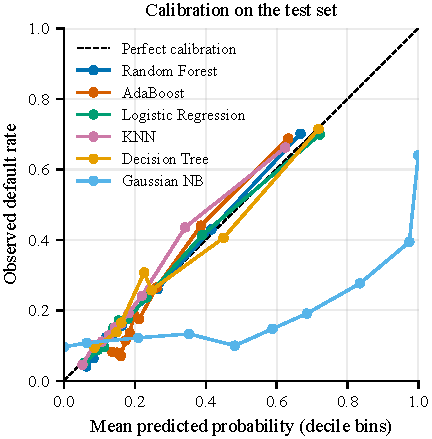
\includegraphics[width=\linewidth]{fig_calibration_test.pdf}
    \caption{Reliability diagrams (decile bins).}
    \label{fig:calib}
  \end{subfigure}\hfill
  \begin{subfigure}[t]{0.46\linewidth}
    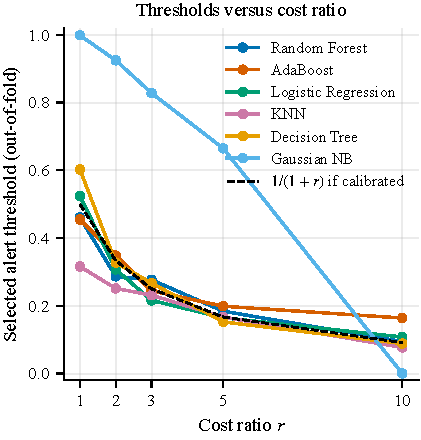
\includegraphics[width=\linewidth]{fig_thresholds_vs_ratio.pdf}
    \caption{OOF-selected thresholds against $1/(1+r)$.}
    \label{fig:thresholds}
  \end{subfigure}
  \caption{Probability quality on the test set and its consequence for thresholds. Models whose scores are calibrated select thresholds close to the theoretical $1/(1+r)$; GNB selects 0.999 at $r=1$ and $6\times10^{-6}$ at $r=10$.}
\end{figure}

\subsection{Thresholds and cost sensitivity}
Figure~\ref{fig:thresholds} shows how the cost-minimising threshold falls as $r$ rises. For the five models with reasonable calibration the thresholds track $1/(1+r)$ (for RF: 0.46, 0.29, 0.28, 0.18, 0.09 against 0.50, 0.33, 0.25, 0.17, 0.09); GNB's thresholds are uninformative as probabilities. Table~\ref{tab:cost} gives the test cost per client at the frozen thresholds for every model and ratio, and Figure~\ref{fig:costimprove} the same numbers relative to the better trivial policy.

Three observations follow. At the primary ratio $r=5$ Random Forest costs 0.553 per client, 29\% below flagging everyone (0.779); the other models save 23--27\%. At $r=10$ the advantage shrinks to 0--11\%: Decision Tree (0.792) is more expensive than flagging everyone and GNB equals it, because at a threshold low enough to catch nearly all defaulters a coarse or miscalibrated score adds nothing. The default threshold 0.5 is costly: at $r=5$ it gives 0.63--0.84 for every model, worse than the trivial policy, because it flags only 11--14\% of clients and misses two thirds of defaulters (Figure~\ref{fig:confusion}); moving RF to its frozen threshold 0.184 raises recall from 0.35 to 0.70 at the price of 1{,}628 extra false alarms and lowers cost from 0.752 to 0.553.

\begin{table}[t]
  \caption{Test cost per client, $C_r(t^\ast)/N$, at the thresholds frozen from out-of-fold predictions. Bold marks the lowest cost per column. The last rows are the trivial policies.}
  \label{tab:cost}
  \centering
  \small
  \begin{tabular}{@{}lccccc@{}}
    \toprule
    & \multicolumn{5}{c}{Cost ratio $r$} \\
    \cmidrule(l){2-6}
    Model & 1 & 2 & 3 & 5 & 10 \\
    \midrule
    Random Forest & 0.179 & 0.307 & \textbf{0.402} & \textbf{0.553} & \textbf{0.695} \\
    AdaBoost & 0.181 & 0.309 & 0.413 & 0.569 & 0.732 \\
    Logistic Regression & 0.179 & \textbf{0.306} & 0.416 & 0.587 & 0.730 \\
    KNN & 0.191 & 0.315 & 0.417 & 0.590 & 0.723 \\
    Decision Tree & \textbf{0.178} & 0.313 & 0.431 & 0.591 & 0.792 \\
    Gaussian NB & 0.193 & 0.332 & 0.431 & 0.599 & 0.779 \\
    \midrule
    Flag no one (majority class) & 0.221 & 0.442 & 0.663 & 1.105 & 2.210 \\
    Flag everyone & 0.779 & 0.779 & 0.779 & 0.779 & 0.779 \\
    \bottomrule
  \end{tabular}
\end{table}

\begin{figure}[htbp]
  \centering
  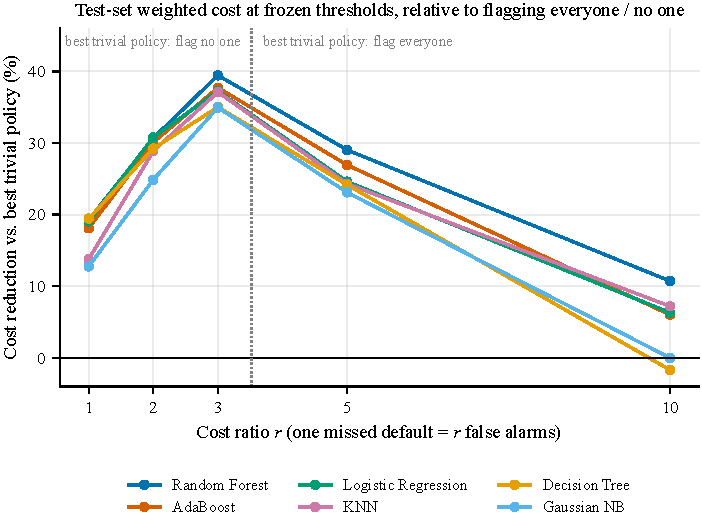
\includegraphics[width=0.78\linewidth]{fig_cost_improvement.pdf}
  \caption{Cost reduction relative to the better trivial policy on the test set. Left of the dotted line the reference is ``flag no one''; right of it, ``flag everyone''.}
  \label{fig:costimprove}
\end{figure}

\subsection{Ranking winner versus operating winner}
\label{sec:rankvscost}
Table~\ref{tab:ranks} places the AP ranking beside the cost ranking at each ratio. Random Forest, first by AP, is cheapest only for $r\ge3$; at $r=1$ the Decision Tree (fifth by AP) is nominally cheapest, at $r=2$ Logistic Regression is, and AdaBoost, second by AP, is fourth by cost at $r=1$ and $r=10$. The bootstrap decides which reversals are real. For $r\le2$ the cost differences between RF, AdaBoost, LR and DT are within $\pm0.01$ per client and every paired interval against RF contains zero, so the four models cannot be separated and the reversal is noise. For $r\ge3$ every interval against RF excludes zero (at $r=5$, RF vs.\ AdaBoost: 0.001--0.031), so RF's advantage is real where the costs are large. Figure~\ref{fig:roc} shows why: the three ROC curves almost coincide near the origin, where the $r=1$ operating points lie, and separate in the middle, where $r=5$ and $r=10$ operate.

\begin{figure}[htbp]
  \centering
  \begin{minipage}[c]{0.44\linewidth}
    \centering
    \footnotesize
    \setlength{\tabcolsep}{3.5pt}
    \begin{tabular}{@{}lcccccc@{}}
      \toprule
      Model & AP & $r{=}1$ & 2 & 3 & 5 & 10 \\
      \midrule
      Random Forest & 1 & 2$^{\circ}$ & 2$^{\circ}$ & 1 & 1 & 1 \\
      AdaBoost & 2 & 4$^{\circ}$ & 3$^{\circ}$ & 2 & 2 & 4 \\
      Logistic Regr. & 3 & 3$^{\circ}$ & 1$^{\circ}$ & 3 & 3 & 3 \\
      KNN & 4 & 5 & 5 & 4 & 4 & 2 \\
      Decision Tree & 5 & 1$^{\circ}$ & 4$^{\circ}$ & 5 & 5 & 6 \\
      Gaussian NB & 6 & 6 & 6 & 6 & 6 & 5 \\
      \bottomrule
    \end{tabular}
    \captionof{table}{Rank by test AP versus rank by test cost at each cost ratio (1 = best). $^{\circ}$: cost difference from Random Forest has a bootstrap interval containing zero.}
    \label{tab:ranks}
  \end{minipage}\hfill
  \begin{minipage}[c]{0.53\linewidth}
    \centering
    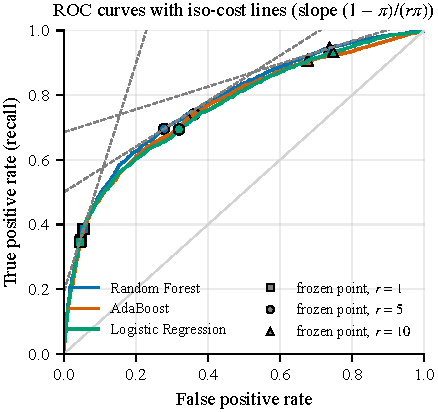
\includegraphics[width=\linewidth]{fig_roc_isocost.pdf}
    \caption{Test ROC curves of the three best-ranking models with frozen operating points for $r=1,5,10$ and iso-cost lines through the Random Forest points.}
    \label{fig:roc}
  \end{minipage}
\end{figure}

Transferring thresholds from out-of-fold predictions to the refitted model cost little: the gap between the frozen-threshold cost and the test-optimal cost is at most 0.013 per client (Decision Tree at $r=10$) and below 0.004 for RF at every ratio except $r=3$ (0.006).

\subsection{What the models use}
All four models that expose importances agree that the most recent repayment status, \texttt{PAY\_0}, dominates (Appendix~\ref{app:features}): it carries 69\% of the Decision Tree's impurity reduction, 48\% of AdaBoost's and 25\% of the Random Forest's, and the four largest LR coefficients are its categories (two months overdue: $+1.05$ log-odds; three months: $+0.98$; code 0: $-1.24$; code $-2$: $-0.96$). Earlier repayment codes and the two most recent payment amounts follow; AdaBoost leans more on payment amounts. The credit limit has a negative coefficient and ranks in the top eight for every tree model. These are predictive associations under the stated preprocessing, not causal effects (Section~\ref{sec:discussion}).

\section{Discussion}
\label{sec:discussion}
\paragraph{Why the best-ranking model need not minimise weighted error.} AP integrates precision over all recall levels, whereas $C_r(t)$ depends on a single point of the ROC curve, the one where the curve's slope equals $(1-\pi)/(r\pi)$~\citep{provost2001robust}. A model can win the integral and lose the point in three ways, and we observe all three. (i) Curves that cross: near the origin the three best ROC curves coincide (Figure~\ref{fig:roc}), so for $r\le2$ no model wins and a simpler one can be nominally cheapest; RF's advantage lies in the middle of the curve, where $r\ge3$ operates. (ii) Threshold transfer: $t^\ast$ is estimated on OOF scores from five fold models and applied to a model refitted on all data; coarse scorers (DT has 109 distinct scores, KNN 162) are most exposed, and DT's regret of 0.013 at $r=10$ is the largest observed. (iii) Noise: with 1{,}990 test defaulters, differences of 0.001--0.003 lie well inside bootstrap intervals, so the $r=1$ ``win'' of the Decision Tree is not evidence. The honest statement is conditional: for $r\ge3$ use Random Forest; for $r\le2$ the four leading models are equivalent and the choice can be made on simplicity and interpretability, which favours Logistic Regression.

\paragraph{From results to a lending decision.} Three qualifications separate ``RF has the lowest cost'' from ``deploy RF at $t=0.184$''. The cost ratio is unknown: 5:1 comes from another dataset and country, and the sensitivity analysis substitutes for knowing it; the recommendation holds for $3\le r\le10$ and not below. As $r$ grows, flagging everyone becomes competitive (the best model saves 11\% at $r=10$), so the question becomes how much review capacity the bank has rather than which classifier to use. Reading scores as probabilities requires calibration: RF, LR and DT qualify, AdaBoost's scores should be rescaled, and GNB's should not be read as probabilities even though its ranking is usable. The negative credit-limit coefficient illustrates causal caution: limits are set by the bank in response to creditworthiness, so it reflects selection, not a protective effect.

\paragraph{Limitations.} In decreasing order of weight. The true cost ratio is unknown; we bounded the conclusion over $r$ but cannot locate it. The data are one Taiwanese issuer in 2005 and the holdout is random, not temporal, so performance in a later period or another market is unassessed. The sample contains only approved cardholders, so the models do not apply to applicants. Thresholds were selected on pooled OOF scores and transferred to refitted models; the measured regret is small ($\le0.013$) but not zero. Grids were small by design and the KNN grid was extended once; $k=201$ lies on a plateau but at the boundary. The repayment codes $-2$ and 0 lack an official definition, impurity importances are not comparable across models, and the Random Forest fixes a leaf size not in the proposal.

\section{Conclusion}
Under one leakage-controlled protocol, Random Forest ranks credit-card defaulters best and, for cost ratios of 3:1 and above, also yields the lowest weighted error; for lower ratios it is statistically tied with Logistic Regression, AdaBoost and a shallow Decision Tree. The larger effect is the threshold, not the model: operating at 0.5 makes every model worse than a trivial policy in the primary scenario, while out-of-fold thresholds for an explicit cost ratio cut cost by a quarter or more. Calibration decides whether those thresholds can be read as probabilities; Gaussian Naive Bayes shows that a usable ranking can coexist with unusable probabilities. The proposal's design held; the instructor's additions turned a single-scenario comparison into a conditional recommendation.

\section*{Member contributions and work plan}
The proposal assigned each member two models and a supporting role; the delivered work followed that plan, with the shared pipeline built first once the feedback compressed the four-week schedule into one. Overall contributions are approximately \textbf{40\% (Shi Xi), 30\% (Li Erteng), 30\% (Jiang Chengrui)}. \textbf{Shi Xi}: Logistic Regression and Gaussian Naive Bayes; data checks, preprocessing and financial interpretation (proposed); in addition, the shared split and evaluation protocol, the cross-validation and freeze-then-test pipeline, calibration and uncertainty analyses, feature interpretation, and drafting and integration of the report (delivered). \textbf{Li Erteng}: KNN and Decision Tree; shared split, cross-validation and experiment records (proposed); verification of the frozen configuration, the experimental-design section, the rank-comparison analysis and the corresponding slides (delivered). \textbf{Jiang Chengrui}: Random Forest and AdaBoost; results visualisation and threshold analysis (proposed); threshold optimisation and cost-sensitivity analysis over five ratios, out-of-fold cost figures, the results section on thresholds and the corresponding slides (delivered). All members reviewed the shared pipeline and contributed to the report and presentation. \todo{confirm wording and percentages with all members}

\bibliographystyle{plainnat}
\bibliography{../references/references}

\clearpage
\appendix
\section{Data dictionary and recoding}
\label{app:data}
\todo{copy the variable table from docs/data\_dictionary.md; add the counts of undocumented codes from docs/data\_check.md}

\section{Hyper-parameter grids and selected configurations}
\label{app:grids}
\begin{table}[h]
  \caption{Pre-stated grids, selected configuration and mean CV AP per candidate. Simpler candidates are listed first and win ties.}
  \centering
  \small
  \begin{tabularx}{\linewidth}{@{}lXl@{}}
    \toprule
    Model & Grid (mean CV AP) & Selected \\
    \midrule
    Logistic Regression & $C\in\{0.1,1,10\}$ $\times$ \texttt{PAY} numeric (0.503, 0.503, 0.503) or one-hot (0.543, 0.544, 0.542) & $C=1$, one-hot \\
    Gaussian NB & default; \texttt{PAY} one-hot tried (0.491 vs.\ 0.487, within fold SD) and not adopted & default \\
    KNN & $k\in\{11,31,61\}$ (0.462, 0.500, 0.512); extended once to $\{101,151,201\}$ (0.515, 0.516, 0.516) & $k=201$ \\
    Decision Tree & depth $\in\{3,5,8\}$ (0.473, 0.511, 0.484) & depth 5 \\
    Random Forest & 200 trees, min.\ 5 per leaf, depth $\in\{5,10,\infty\}$ (0.551, 0.557, 0.552) & depth 10 \\
    AdaBoost & 100 stumps, rate $\in\{0.1,0.5,1\}$ (0.536, 0.536, 0.535) & rate 0.1 \\
    \bottomrule
  \end{tabularx}
\end{table}

\section{Decision metrics at the primary scenario}
\label{app:decisions}
\begin{table}[h]
  \caption{Test-set confusion counts and derived metrics at the frozen threshold for $r=5$ ($N=9{,}003$, 1{,}990 defaulters).}
  \centering
  \small
  \begin{tabular}{@{}lccccccccc@{}}
    \toprule
    Model & $t^\ast$ & TP & FP & FN & TN & Precision & Recall & Error rate & Cost/client \\
    \midrule
    Random Forest & 0.184 & 1385 & 1952 & 605 & 5061 & 0.415 & 0.696 & 0.284 & 0.553 \\
    AdaBoost & 0.199 & 1474 & 2544 & 516 & 4469 & 0.367 & 0.741 & 0.340 & 0.569 \\
    Logistic Regression & 0.165 & 1381 & 2242 & 609 & 4771 & 0.381 & 0.694 & 0.317 & 0.587 \\
    KNN & 0.167 & 1404 & 2378 & 586 & 4635 & 0.371 & 0.706 & 0.329 & 0.590 \\
    Decision Tree & 0.152 & 1530 & 3018 & 460 & 3995 & 0.336 & 0.769 & 0.386 & 0.591 \\
    Gaussian NB & 0.665 & 1316 & 2023 & 674 & 4990 & 0.394 & 0.661 & 0.300 & 0.599 \\
    \bottomrule
  \end{tabular}
\end{table}

\begin{figure}[h]
  \centering
  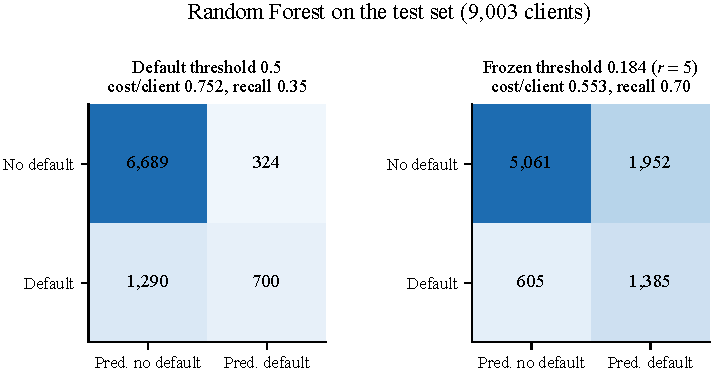
\includegraphics[width=\linewidth]{fig_confusion_rf.pdf}
  \caption{Random Forest confusion matrices on the test set at the default and the frozen ($r=5$) threshold.}
  \label{fig:confusion}
\end{figure}

\section{Feature interpretation}
\label{app:features}
\begin{figure}[h]
  \centering
  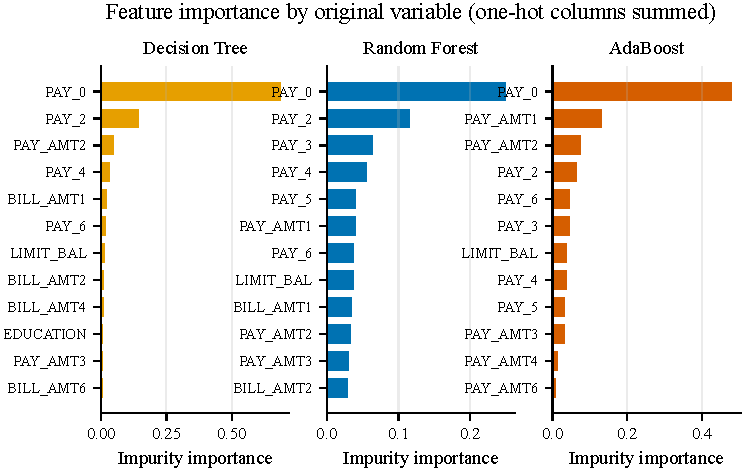
\includegraphics[width=\linewidth]{fig_feature_importance.pdf}
  \caption{Impurity-based importance by original variable (one-hot columns summed) for the three tree models fitted on the full development set.}
\end{figure}
\begin{figure}[h]
  \centering
  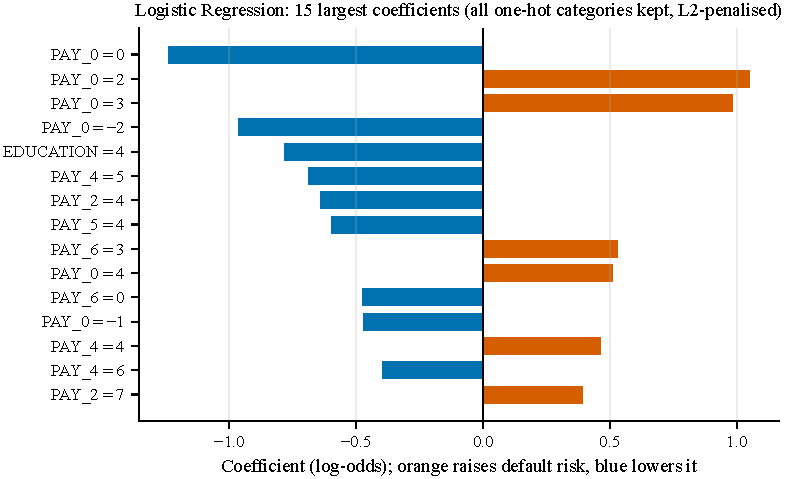
\includegraphics[width=\linewidth]{fig_feature_logistic.pdf}
  \caption{Fifteen largest Logistic Regression coefficients. All one-hot categories are retained under L2 regularisation, so each coefficient is relative to the average of its variable's categories, not to an omitted baseline.}
\end{figure}

\section{Additional figures}
\begin{figure}[h]
  \centering
  \begin{subfigure}[t]{0.45\linewidth}
    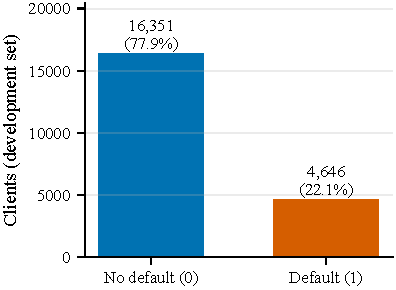
\includegraphics[width=\linewidth]{fig_class_balance.pdf}
    \caption{Class balance in the development set.}
  \end{subfigure}\hfill
  \begin{subfigure}[t]{0.5\linewidth}
    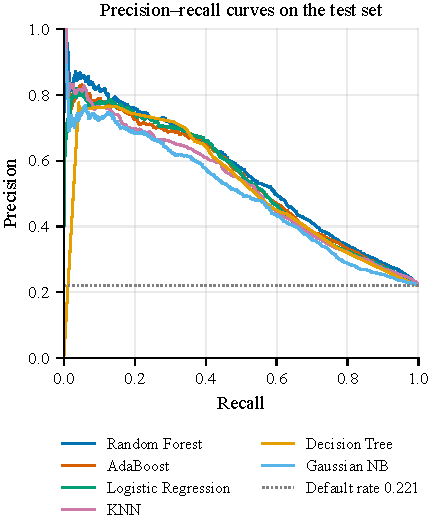
\includegraphics[width=\linewidth]{fig_pr_curves.pdf}
    \caption{Precision--recall curves on the test set.}
  \end{subfigure}
  \caption{Supporting figures.}
\end{figure}

\section{Reproducibility}
The repository contains the raw file (SHA-256 recorded), the split indices, every out-of-fold and test prediction, the frozen configuration with its commit hash, the fitted pipelines and the scripts \texttt{01}--\texttt{10} that regenerate every table and figure in this report. Package versions are pinned (\texttt{scikit-learn} 1.9.1, \texttt{numpy} 2.5.4); the Random Forest results change in the third decimal under other versions. \texttt{python -m pytest} checks the split and the metric functions.

\end{document}
